% Filename: Results
% Last update: Monday, 12/17/2018 by Ally Warner
%
%%%%%%%%%%%%%%%%%%%%%%%%%%%%%%%%%%%%%%%%%%%%%%%%%%%%%%%%%%%%%%%%%%%%%%

\section{Results}
\label{sec:results}

All SCIRun networks used to generate results are included in an open-source dataset for research use at \url{www.sci.utah.edu/SCI_headmodel}. Details of this dataset are described in Table \ref{tab:res}.

%Table of what's included in the dataset or itemized list 
%a complete, high-resolution brain segmentation that can be used to create three-dimensional tetrahedral volume and surface meshes. We provide two three-dimensional tetrahedral finite element meshes made from the segmentation of different resolutions that serve as volume conductors to solve forward and inverse EEG problems. We also provide simulation examples of the EEG forward problem, with isotropic and anisotropic systems; functional image data mapped onto a tetrahedral mesh; electroencephalography (EEG) signals mapped onto net electrodes; and diffusion tensor data.

\subsection{Segmentation}

For this project, we segmented the head into eight detailed layers, listed in Section \ref{sec:Seg}. We used this segmentation to create an inhomogeneous three-dimensional tetrahedral mesh.

\begin{figure}[H]
\begin{center}
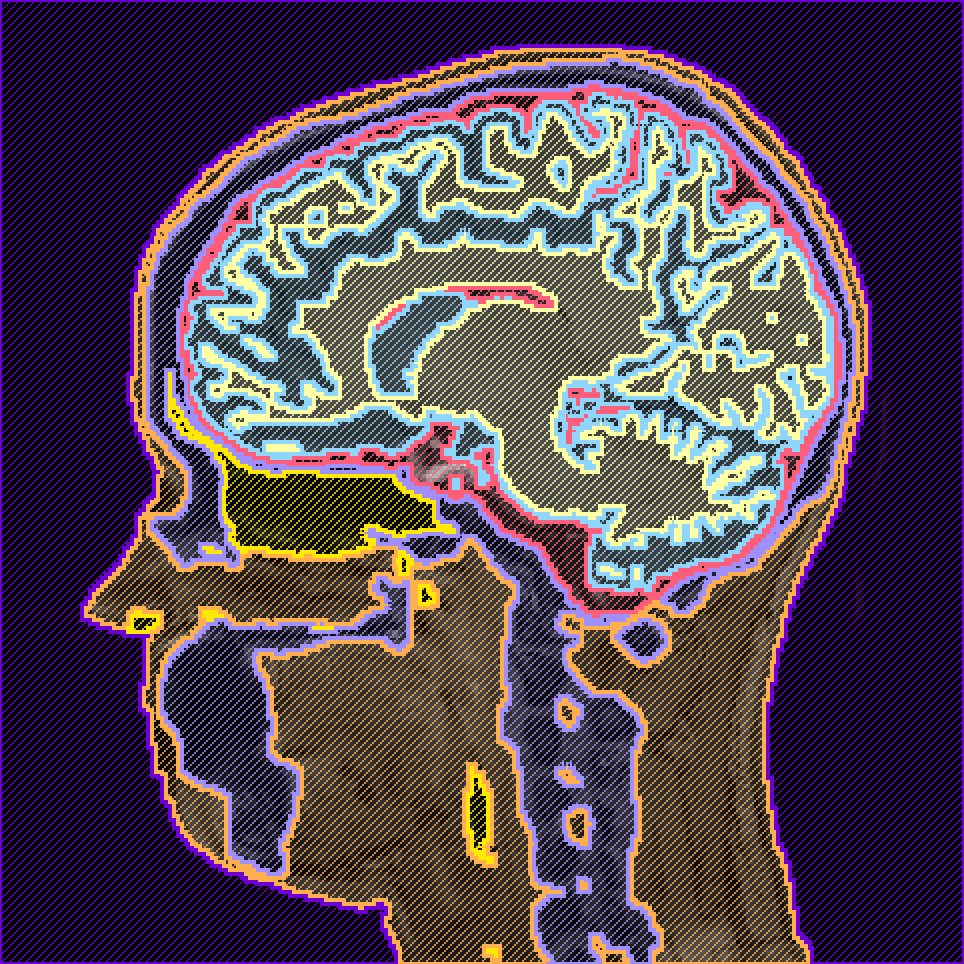
\includegraphics[height=2.35in]{Figures/seg_1}
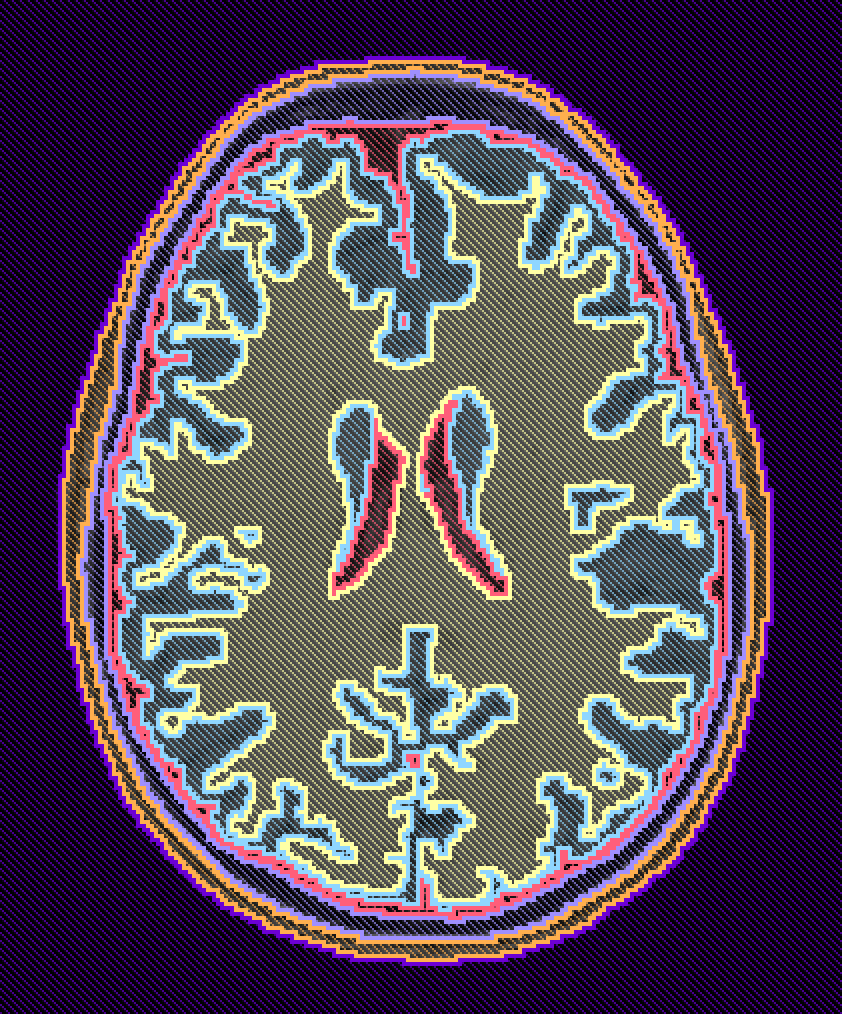
\includegraphics[height=2.35in]{Figures/seg_2}
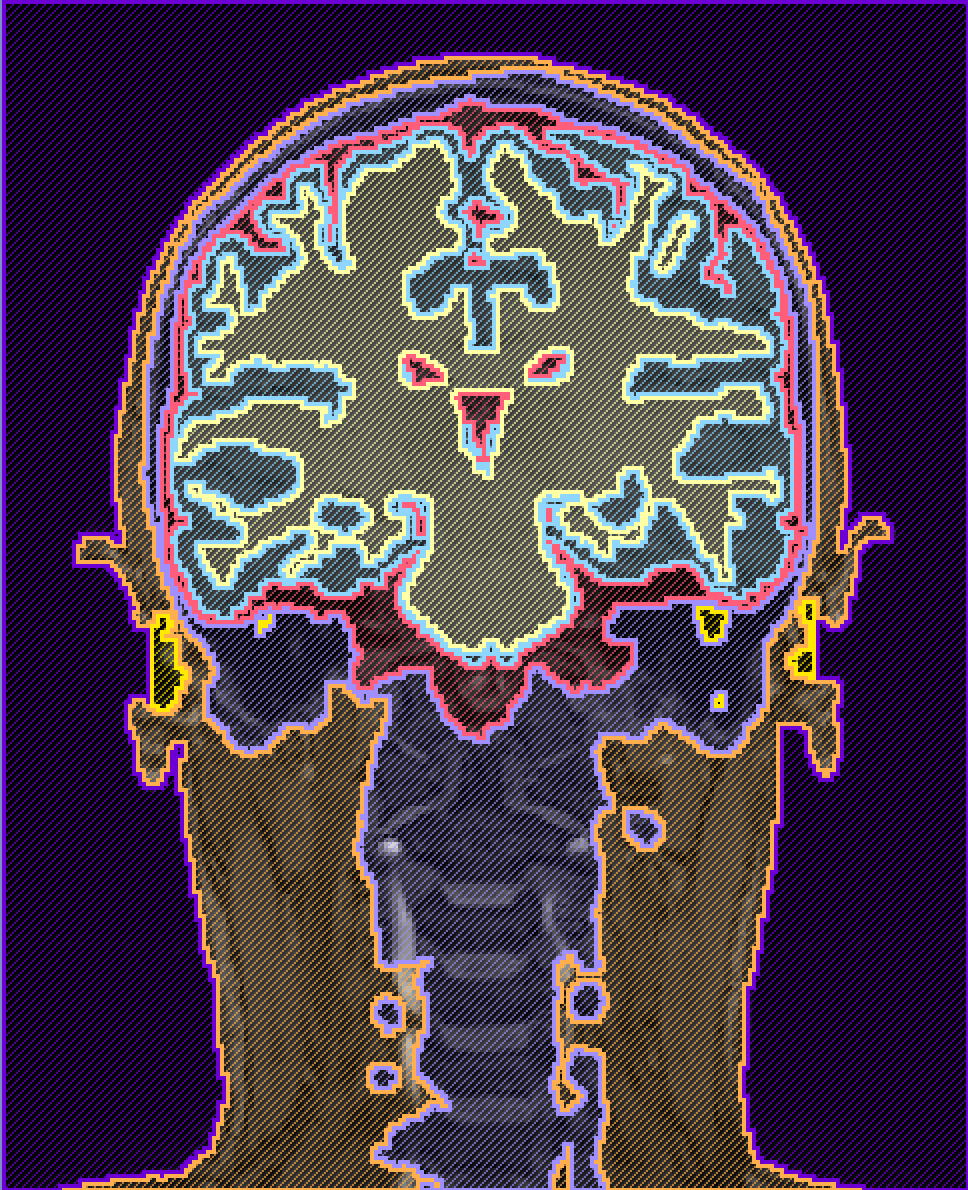
\includegraphics[height=2.35in]{Figures/seg_3}
\caption{A high-resolution, eight-layer, full head segmentation made with Seg3D.}
\label{fig:fullseg}
\end{center}
\end{figure}

The two bone segmentation methods, discussed in Section \ref{sec:Seg}, produced geometries that were similar in some areas, but different in others. The segmentation created using FSL and Seg3D was rough and had a clear line of where the two segmentations were connected. It also didn't include a chin or a sinus layer. The segmentation created from the pseudo-CT scan was smooth and included a chin and a sinus layer. This segmentation did include the inside of the mouth as bone, but as mentioned before this wasn't concerning for simulations results.

\begin{figure}[H]
\begin{center}
\includegraphics[width=.49\textwidth]{Figures/skull_before}
\includegraphics[width=.49\textwidth]{Figures/skull_after}
\caption{Skull segmentation comparison: Created with BET and thresholding \textit{(left)} and with pseudo-CT \textit{(right)}. Both segmentations were made using Seg3D.}
\label{fig:skull}
\end{center}
\end{figure}

\begin{figure}[H]
\begin{center}
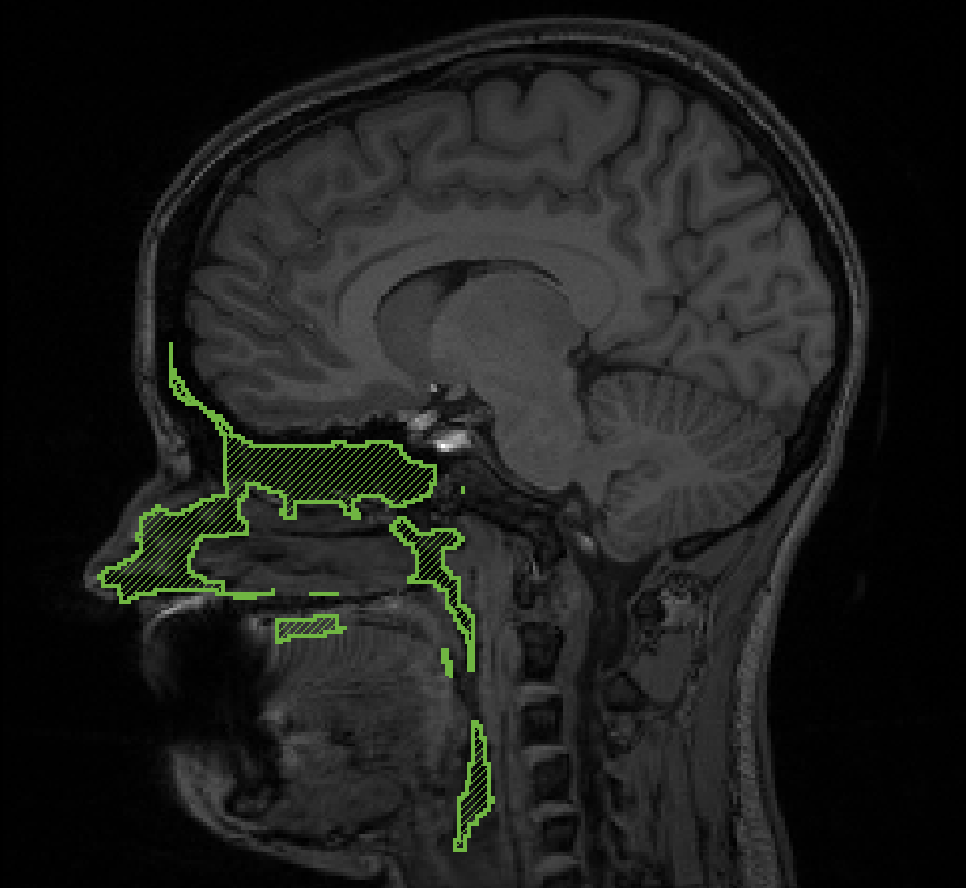
\includegraphics[width=.49\textwidth]{Figures/sinus_sag}
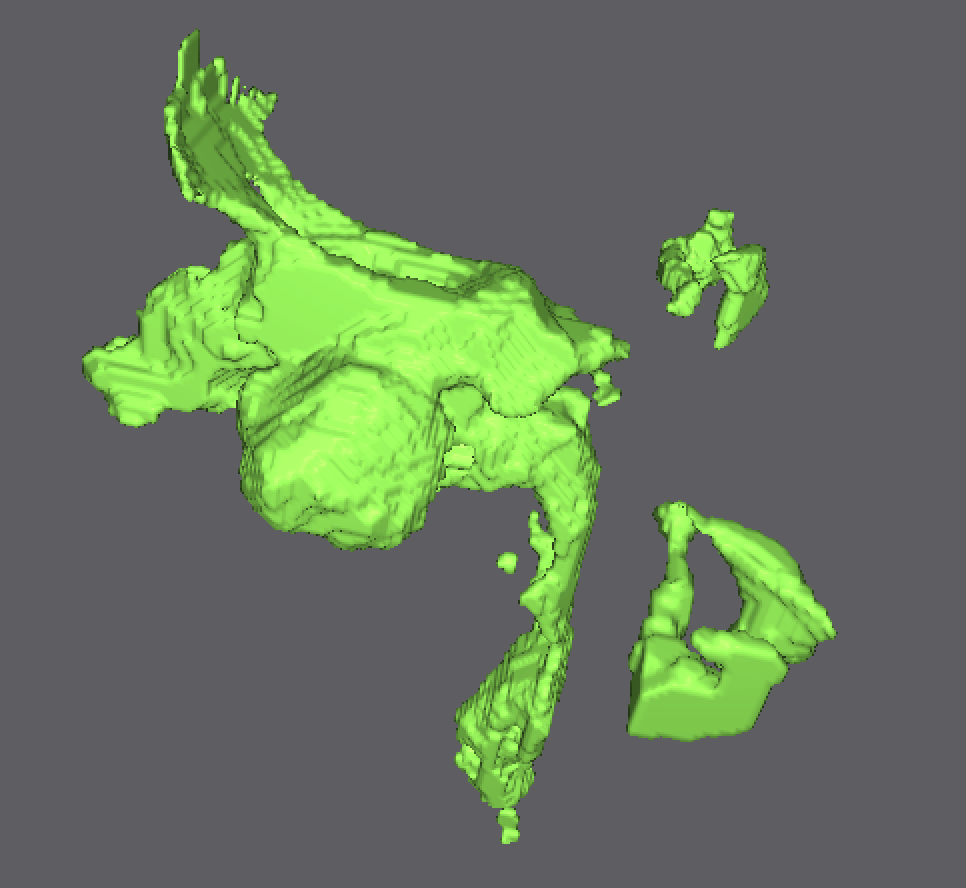
\includegraphics[width=.49\textwidth]{Figures/sinus_iso}
\caption{Sinus segmentation.}
\label{fig:sinus}
\end{center}
\end{figure}

During MRI imaging, the subject was on her back, which caused the brain to shift to the back of the head, resulting in thin segmented sections on the back of the head as well as on the side of the subject's head, the bridge of the nose, and the bottom of the chin. We made these sections at least two pixels thick to ensure a mesh without holes.

\begin{figure}[H]
\begin{center}
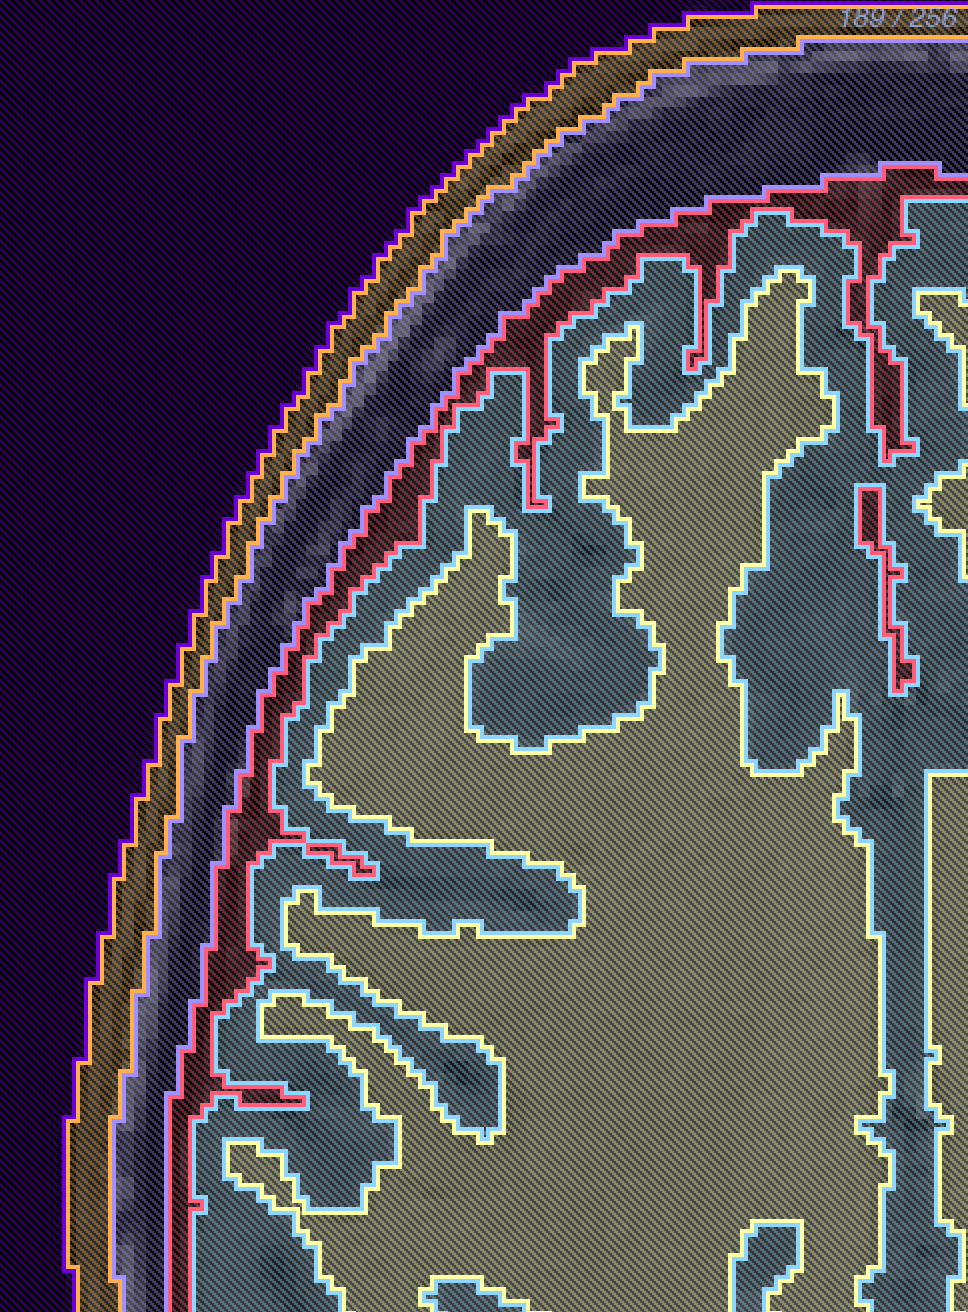
\includegraphics[width=.32\textwidth]{Figures/thin_layer_side}
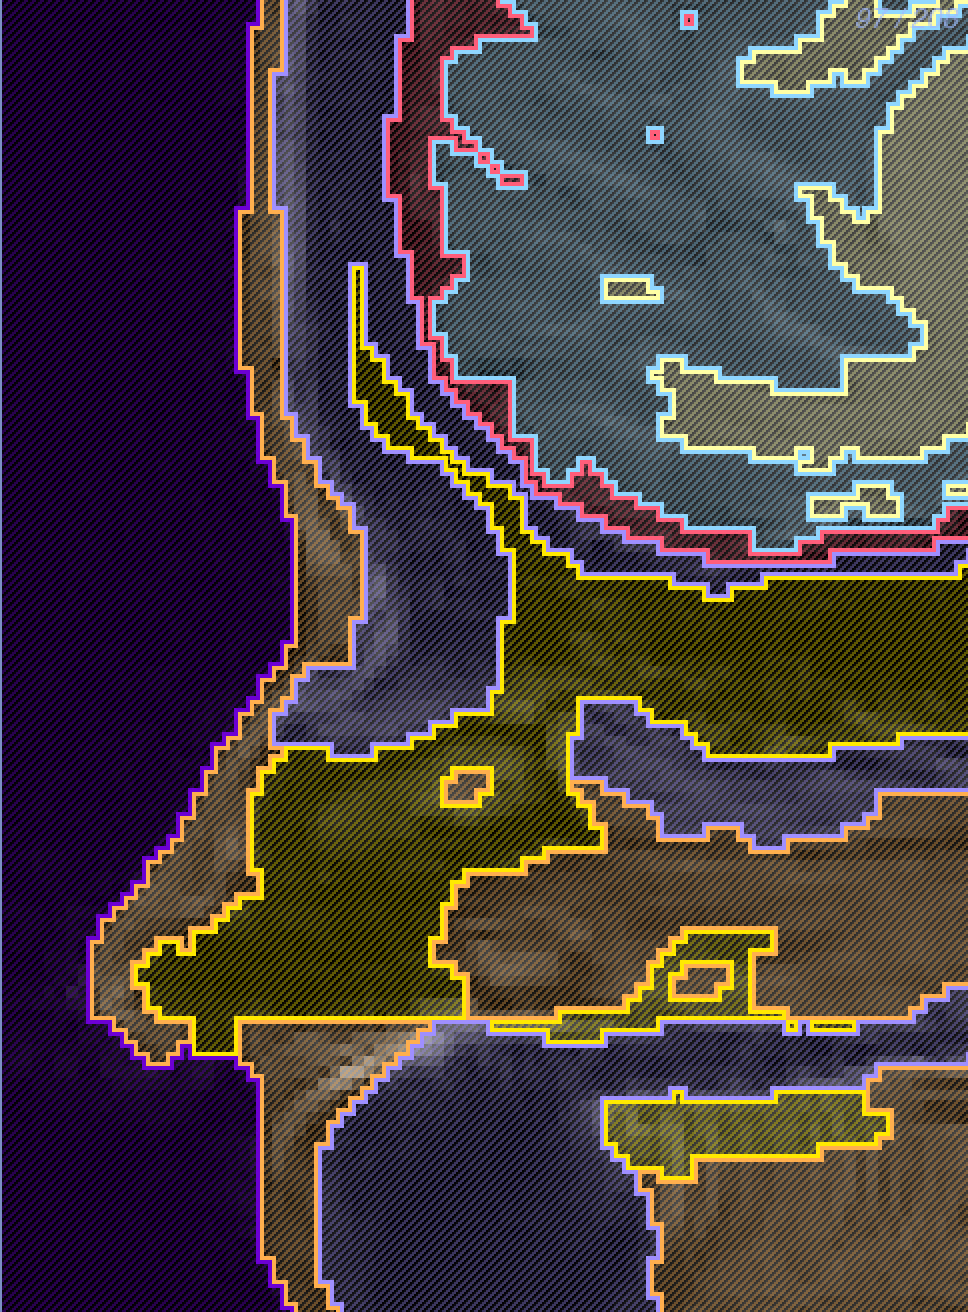
\includegraphics[width=.32\textwidth]{Figures/thin_layer_nose}
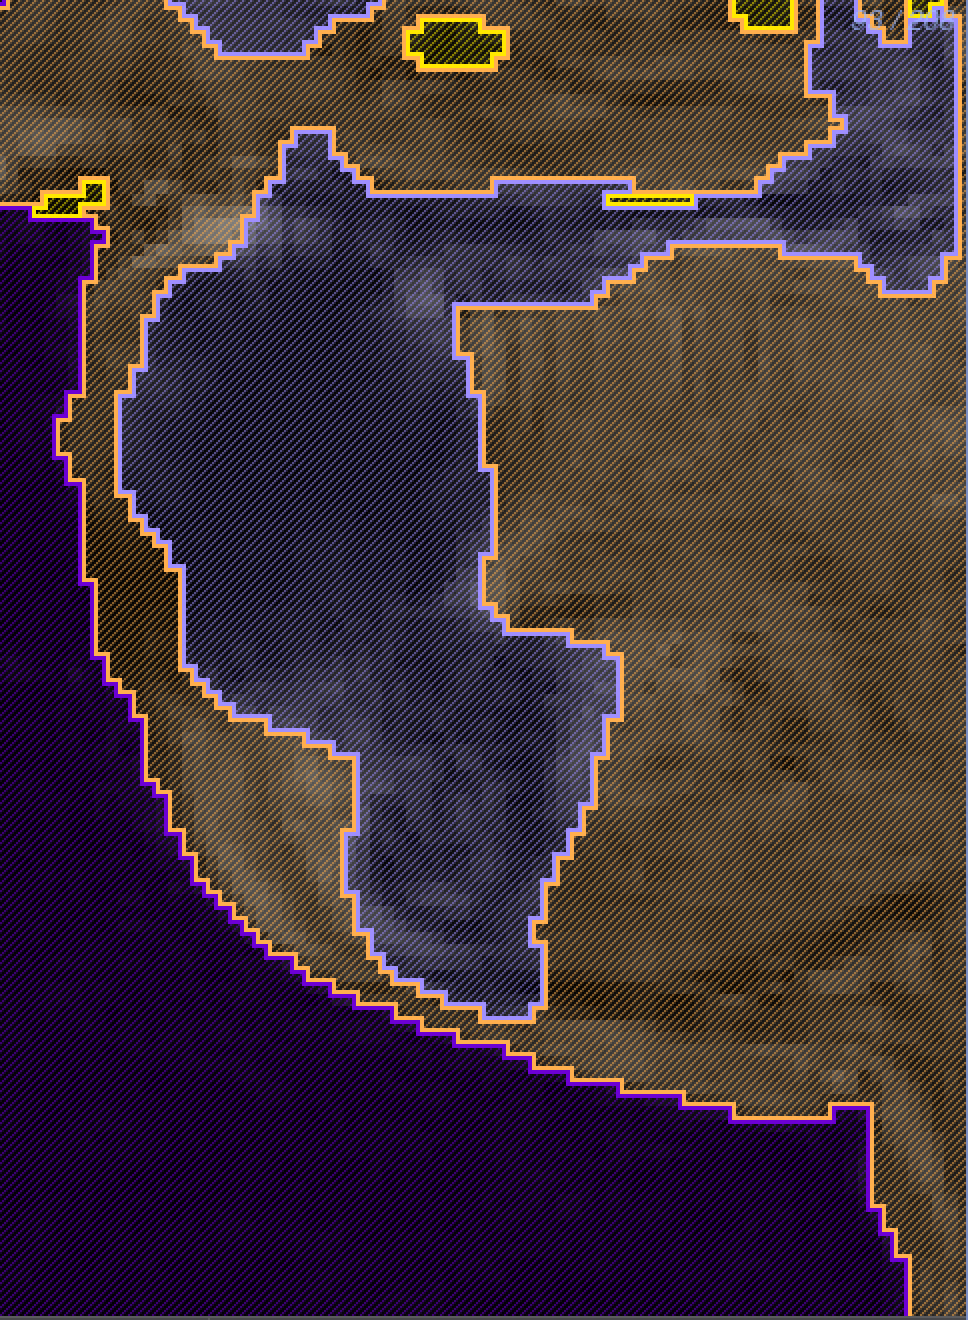
\includegraphics[width=.32\textwidth]{Figures/thin_layer_chin}
\caption{Thin segmentation sections: side of the head \textit{(left)}, bridge of the nose \textit{(middle)}, bottom of the chin \textit{(right)}.}
\label{fig:thinseg}
\end{center}
\end{figure}


%%EXTRAS TO PUT IN
 Segmentation of the brain was difficult because of the similar grayscale intensities across different tissues; thresholding the image produced noisy and incomplete layers. Segmentation of the sinuses and skull was also difficult because they are represented by only black pixels, with no clear tissue boundaries.

This method, compared with Freesurfer \cite{ref:freesurf}, Statistical Parametric Mapping through Matlab (SPM) \cite{ref:spm}, Atlas Based Classification through 3D Slicer \cite{ref:abc}, and Seg3D methods alone, produced the most qualitatively accurate initial brain segmentation results for this data.

\subsection{Finite Element Meshes}

The highest resolution mesh we generated with the settings listed in Section \ref{sec:mesh} had 60.2 million elements and 10.3 million nodes. This mesh was large because of the complexity of the segmentation, including small features, thin sections, and several layers touching at once. The simulations performed slowly when using this mesh due to its size and required at least 32GB of RAM.

\begin{figure}[H]
\begin{center}
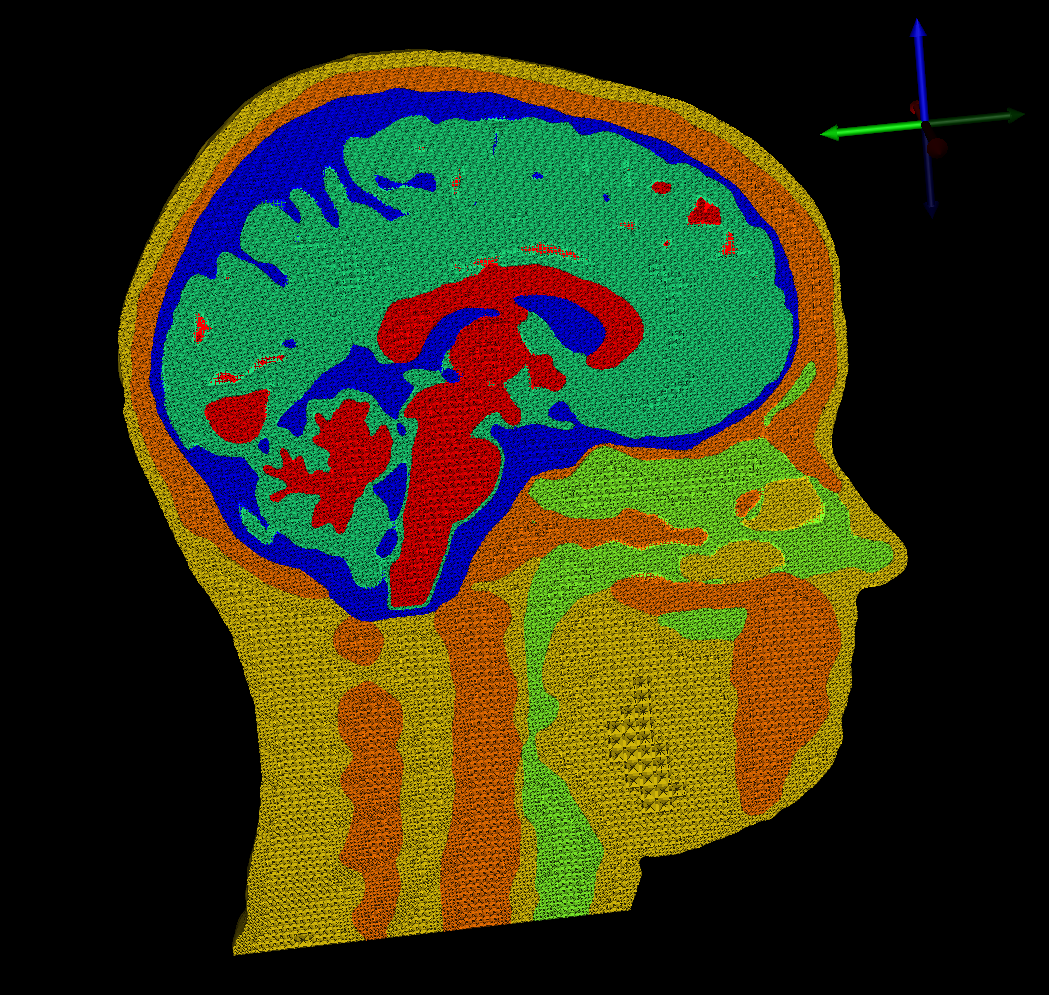
\includegraphics[width=.49\textwidth]{Figures/bigmesh_1}
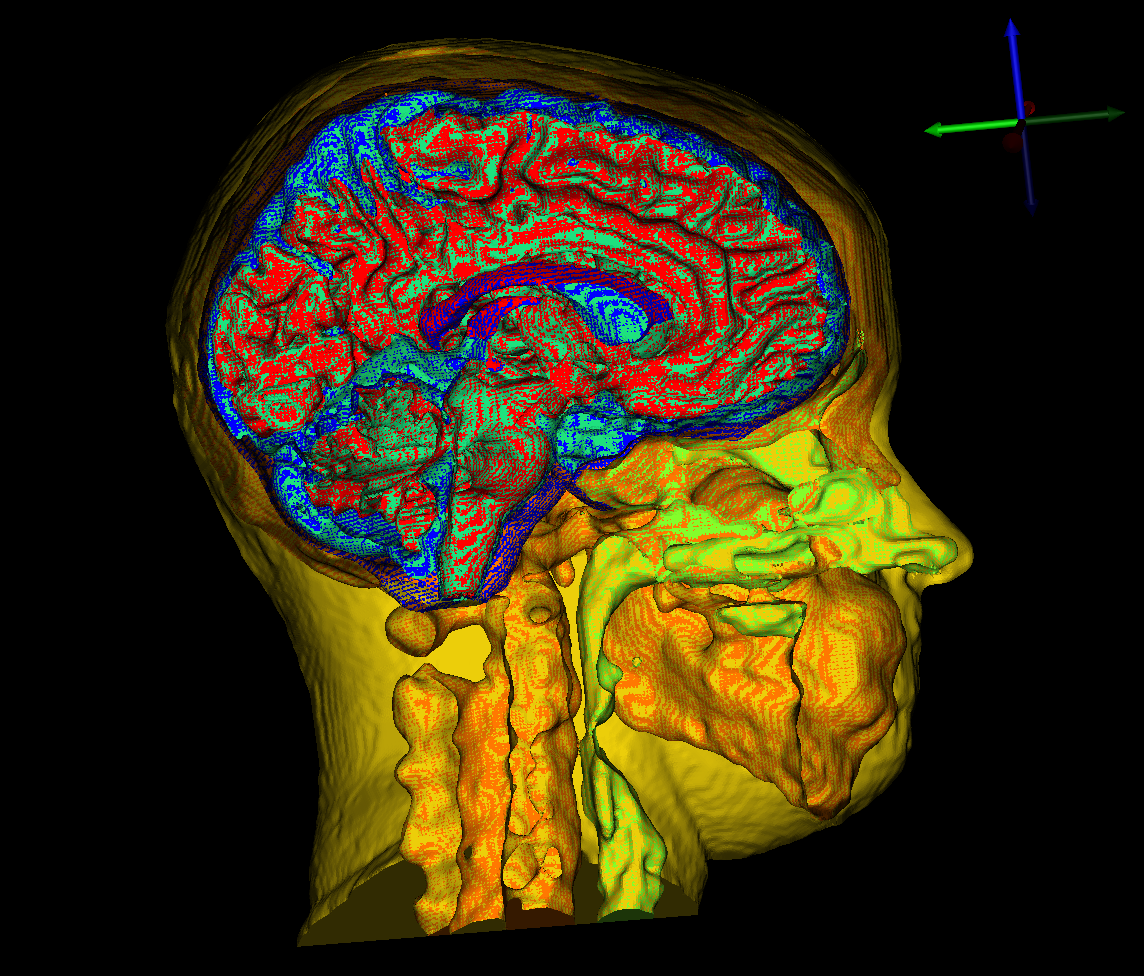
\includegraphics[width=.49\textwidth]{Figures/bigmesh_surface}
\caption{60.2 M element mesh: tetrahedral mesh \textit{(left)}, surface mesh \textit{(right)}.}
\label{fig:bigmesh}
\end{center}
\end{figure}

We attempted to generate smaller meshes to be able to run quicker simulations, but many of the meshes contained holes. After we manually changed the sizing field described in Section \ref{sec:mesh}, we generated a mesh with 15.7 million elements and 2.7 million nodes without holes. However, this mesh contained one flat tetrahedra, which we later removed in a SCIRun network. This issue is currently being investigated by Cleaver software developers.

\begin{figure}[H]
\begin{center}
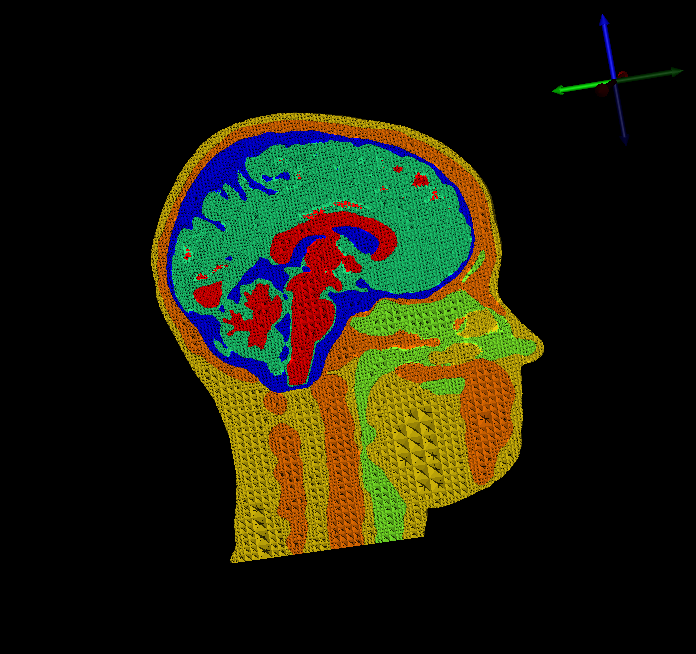
\includegraphics[width=.49\textwidth]{Figures/smallmesh_2}
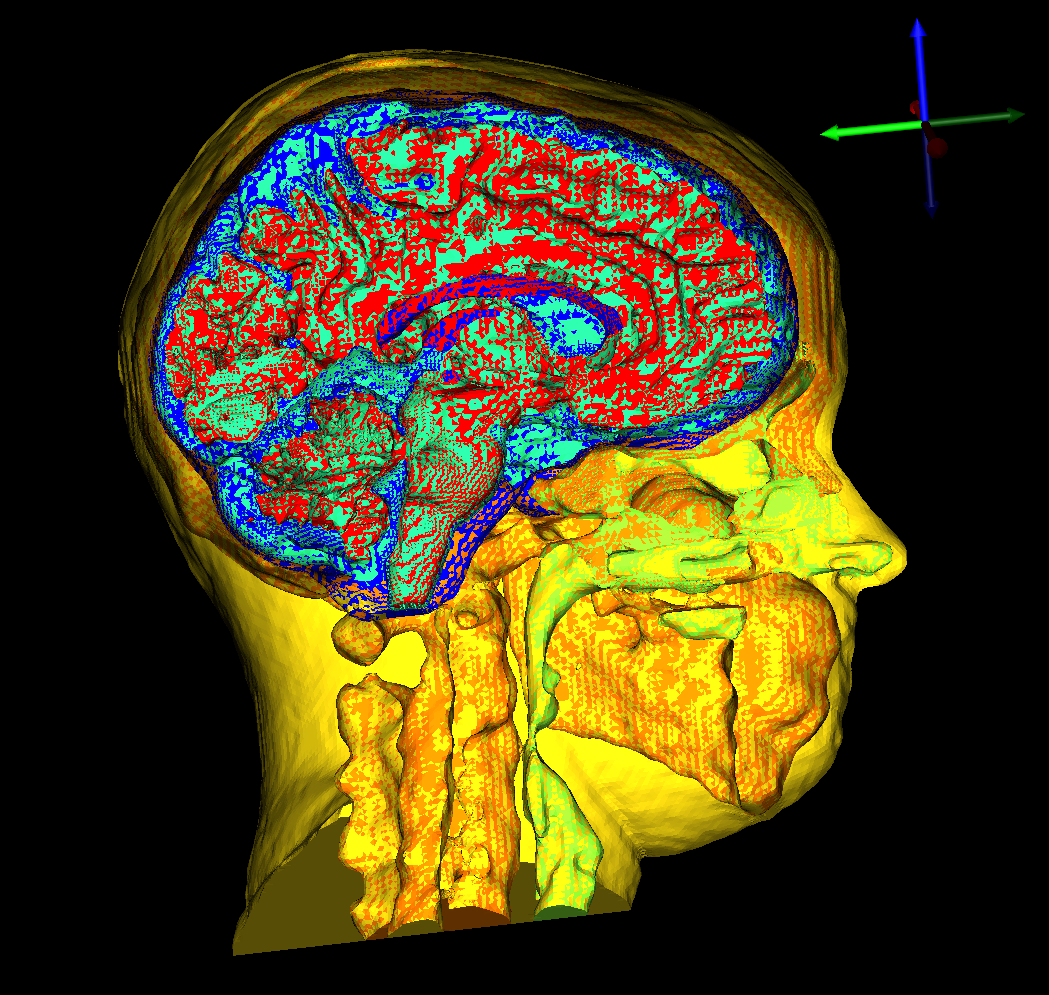
\includegraphics[width=.49\textwidth]{Figures/smallmesh_surface}
\caption{15.7 M element mesh: tetrahedral mesh \textit{(left)}, surface mesh \textit{(right)}.}
\label{fig:smallmesh}
\end{center}
\end{figure}

\subsection{Diffusion Tensor Images}
\begin{figure}[H]
\begin{center}
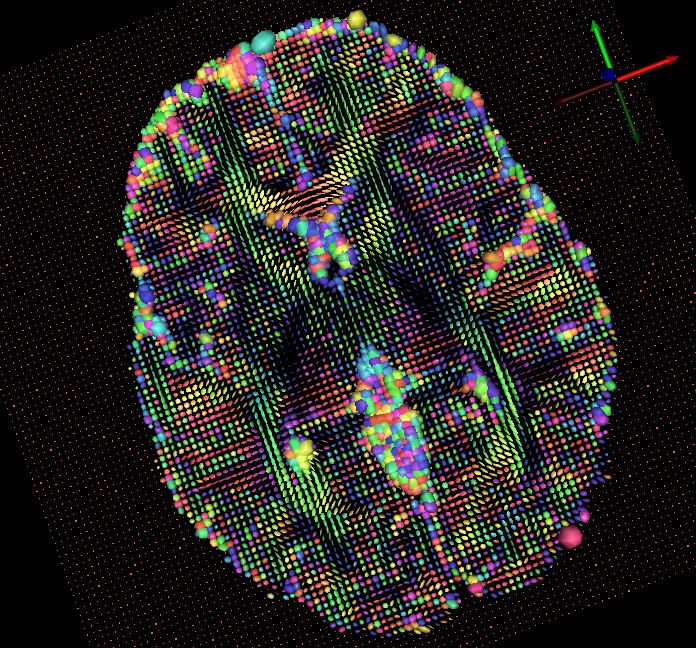
\includegraphics[width=0.75\textwidth]{Figures/DTI_1.png}
\caption{Diffusion tensor visualization using SCIRun.}
\label{fig:tensorvis}
\end{center}
\end{figure}

\begin{figure}[H]
\begin{center}
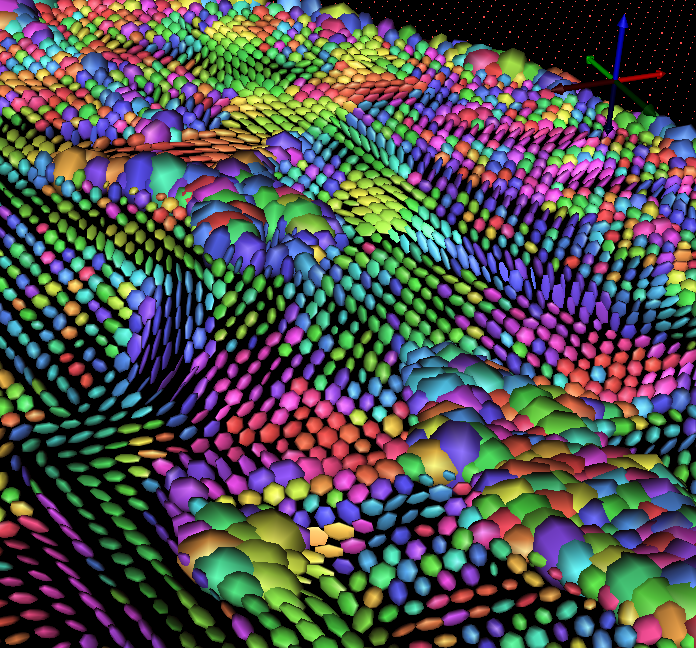
\includegraphics[width=0.75\textwidth]{Figures/DTI_2.png}
\caption{Diffusion tensor visualization using SCIRun.}
\label{fig:tensorvis2}
\end{center}
\end{figure}

We built the tensor field in SCIRun rather than in 3D Slicer \cite{ref:slicer} or FSL DTIFIT because the output data had a different orientation and could not be easily registered with the mesh in SCIRun.

\begin{figure}[H]
\begin{center}
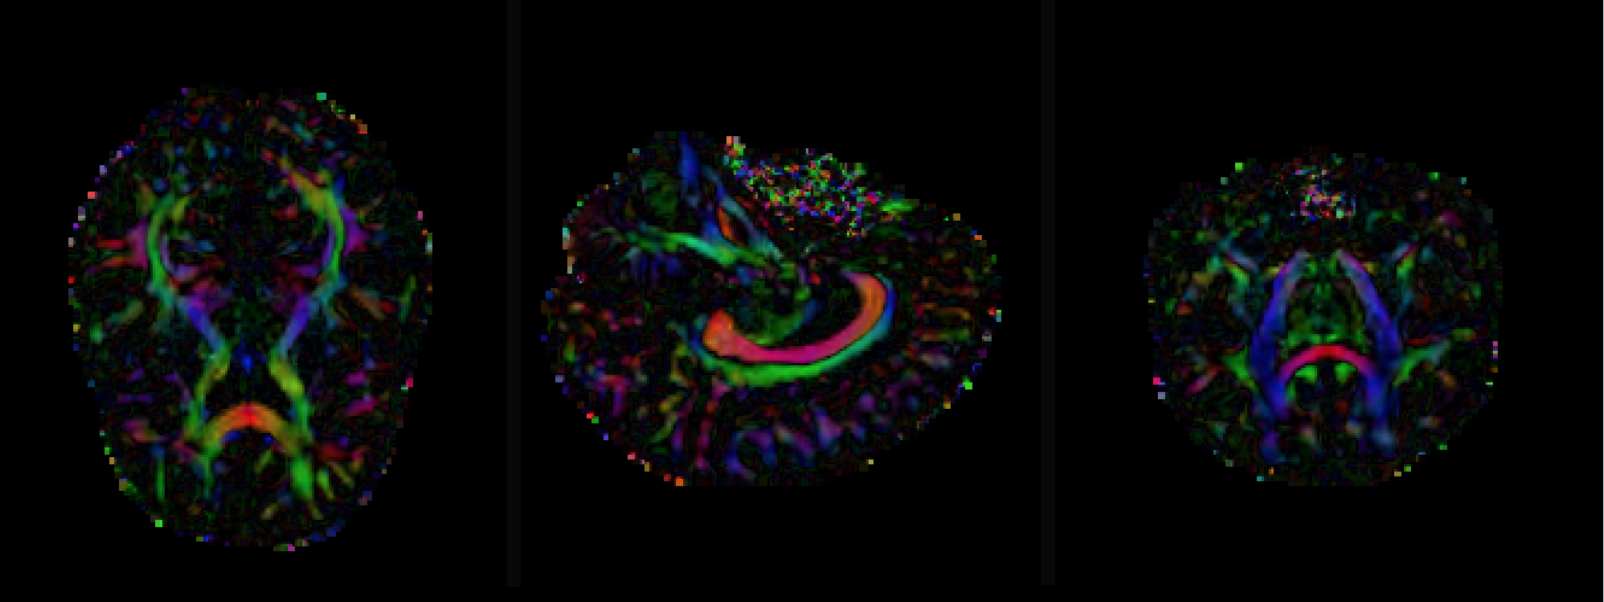
\includegraphics[width=0.75\textwidth]{Figures/backwards.png}
\caption{Example of difference in orientation between SCIRun and 3D
  Slicer data.}
\label{fig:backwards}
\end{center}
\end{figure}

\subsection{Forward Problem}

\subsubsection{Isotropic}

An isotropic, inhomogeneous head model is expected to have largely spherical propagation of electrical signals. We generated three-dimensional streamlines as well as isopotential lines to visualize this propagation and to compare isotropic and anisotropic conductivity. The simulations showed spherical propagation and acceptable registration of electrodes and dipoles to the mesh space.

\begin{figure}[H]
\begin{center}
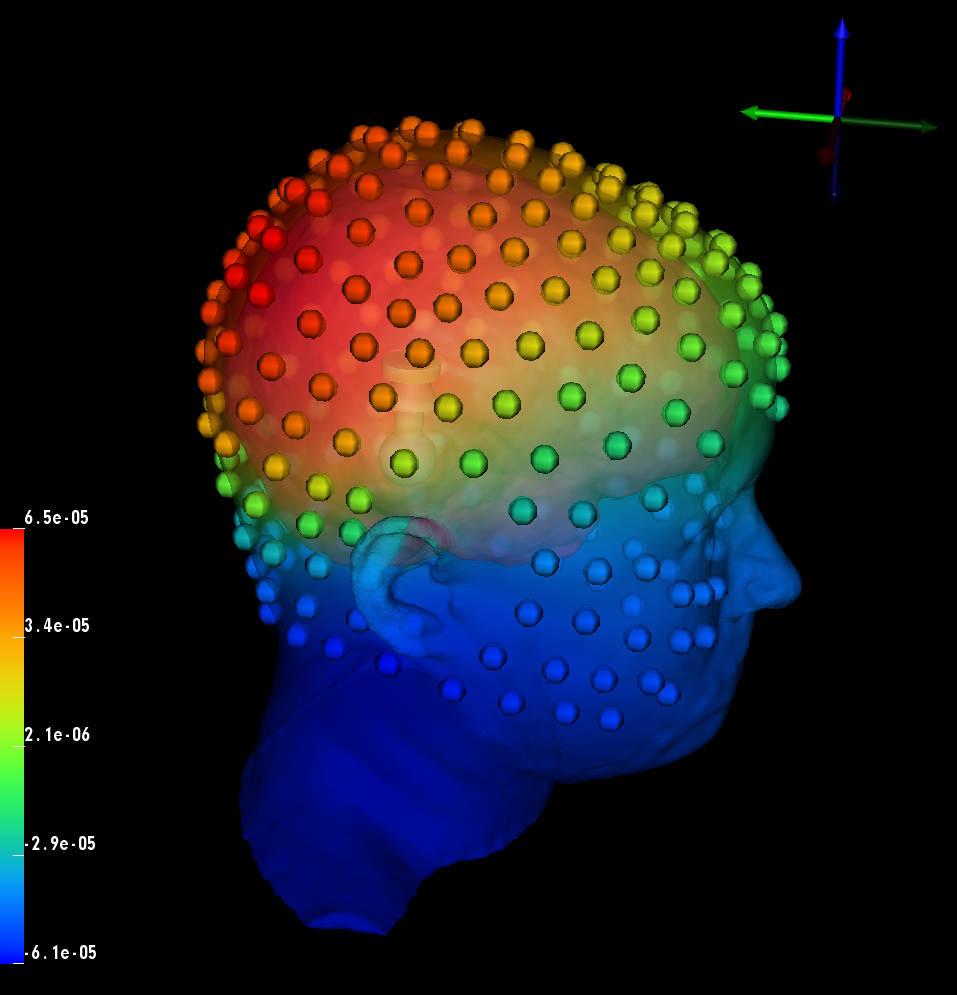
\includegraphics[width=.49\textwidth]{Figures/iso_dipole}
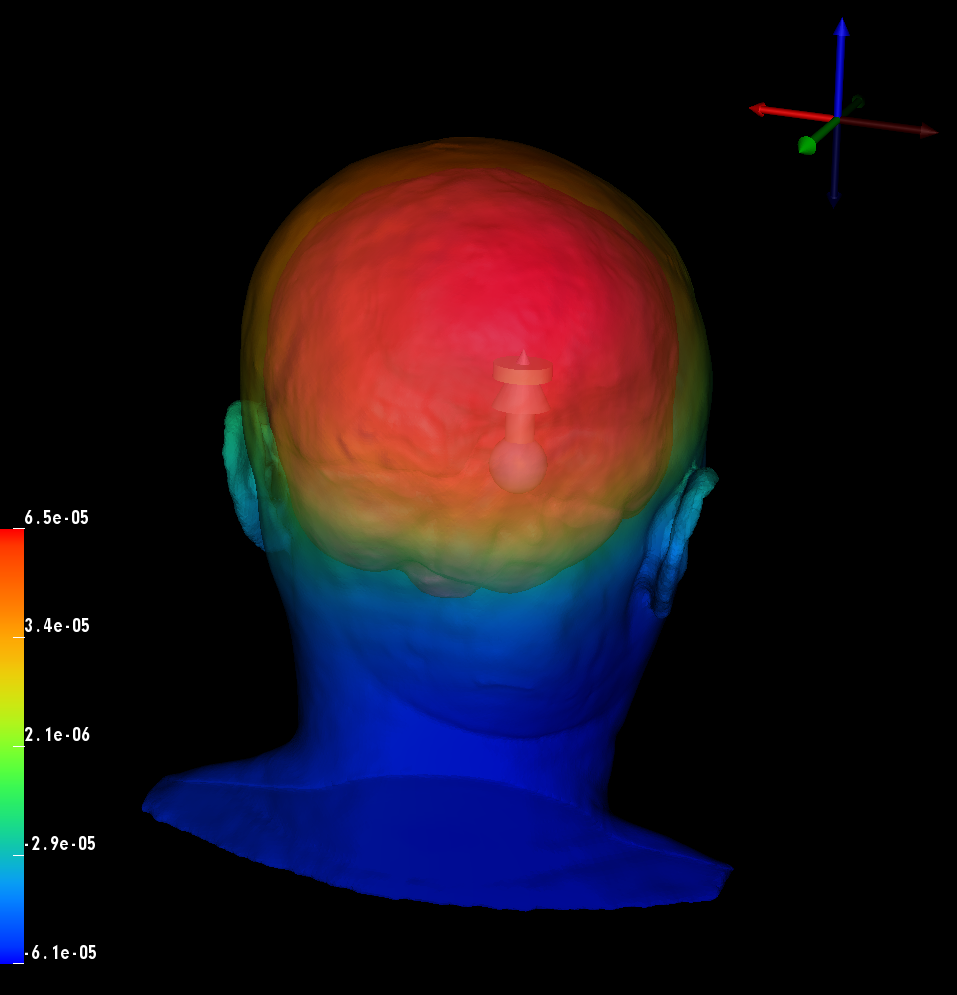
\includegraphics[width=.49\textwidth]{Figures/iso_dipole_2}
\caption{Isotropic forward problem solution with dipole source and data mapped onto the head surface and electrodes.}
\label{fig:isodip}
\end{center}
\end{figure}

\begin{figure}[H]
\begin{center}
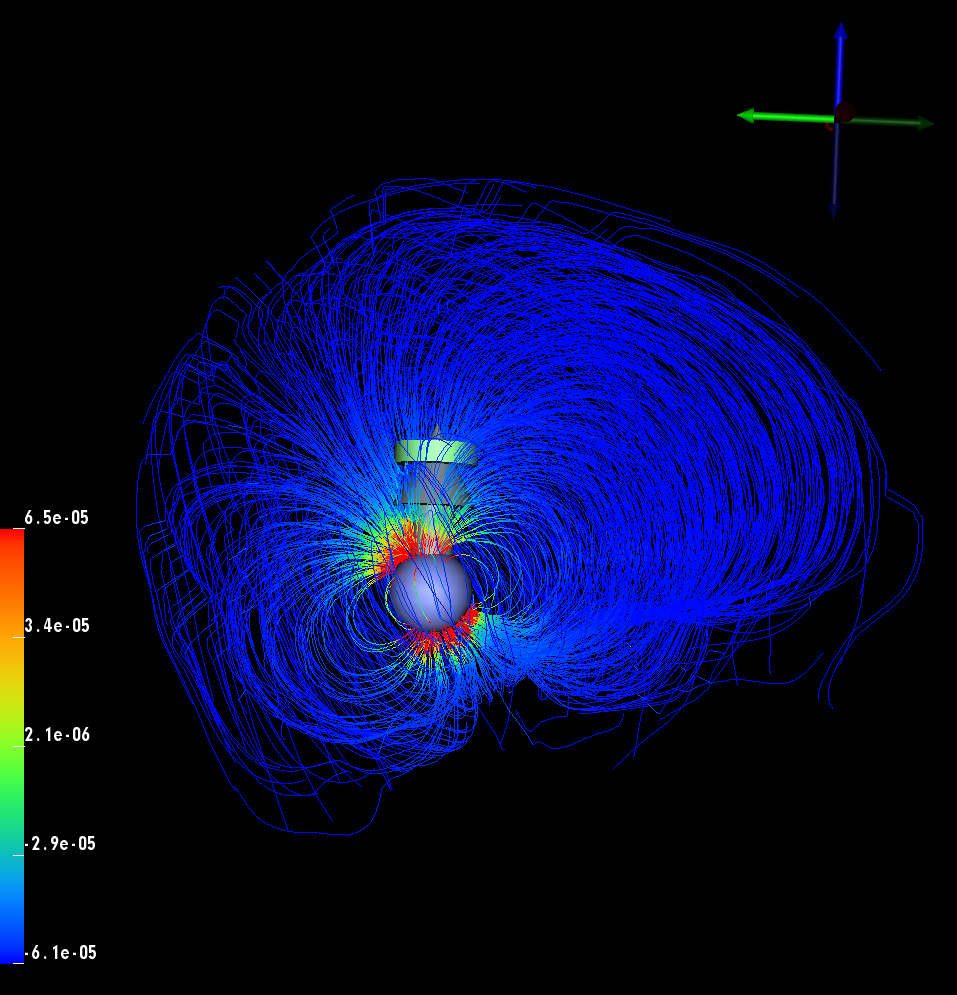
\includegraphics[width=.49\textwidth]{Figures/iso_streamlines}
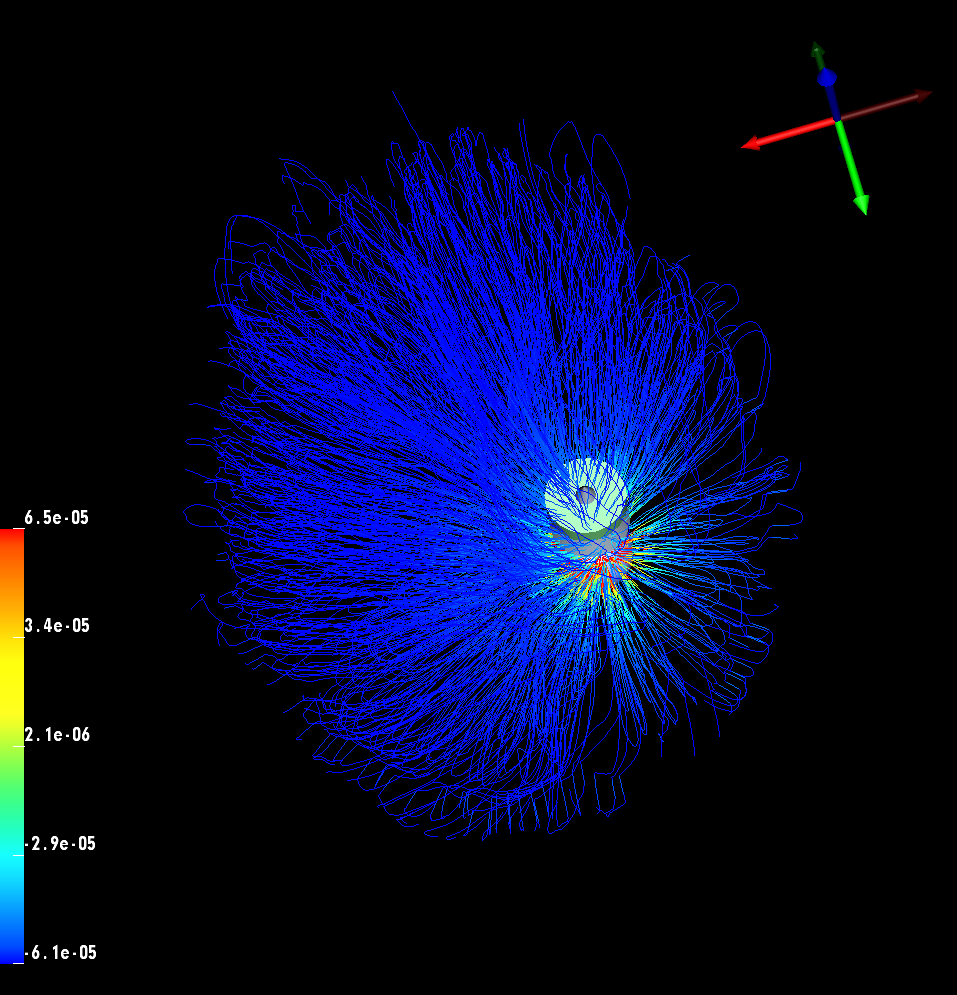
\includegraphics[width=.49\textwidth]{Figures/iso_streamlines_top}
\caption{Isotropic streamlines with dipole source.}
\label{fig:isostream}
\end{center}
\end{figure}

\subsubsection{Anisotropic}

The expectation for an anisotropic, inhomogeneous head model is to have nonspherical propagation, which can be seen with the streamline and isoline visualizations. As discussed in Section \ref{sec:cond}, two methods are used for implementing diffusion tensor data, both being available in the SCIRun network shown in Figure \ref{fig:anisofornet}. For Figures \ref{fig:anisodip} - \ref{fig:isolines}, we used the scaling method (equation \ref{eq:scaling}). The simulations showed nonspherical propagation and acceptable registration of the electrodes, dipoles, and mesh into the diffusion tensor space.

\begin{figure}[H]
\begin{center}
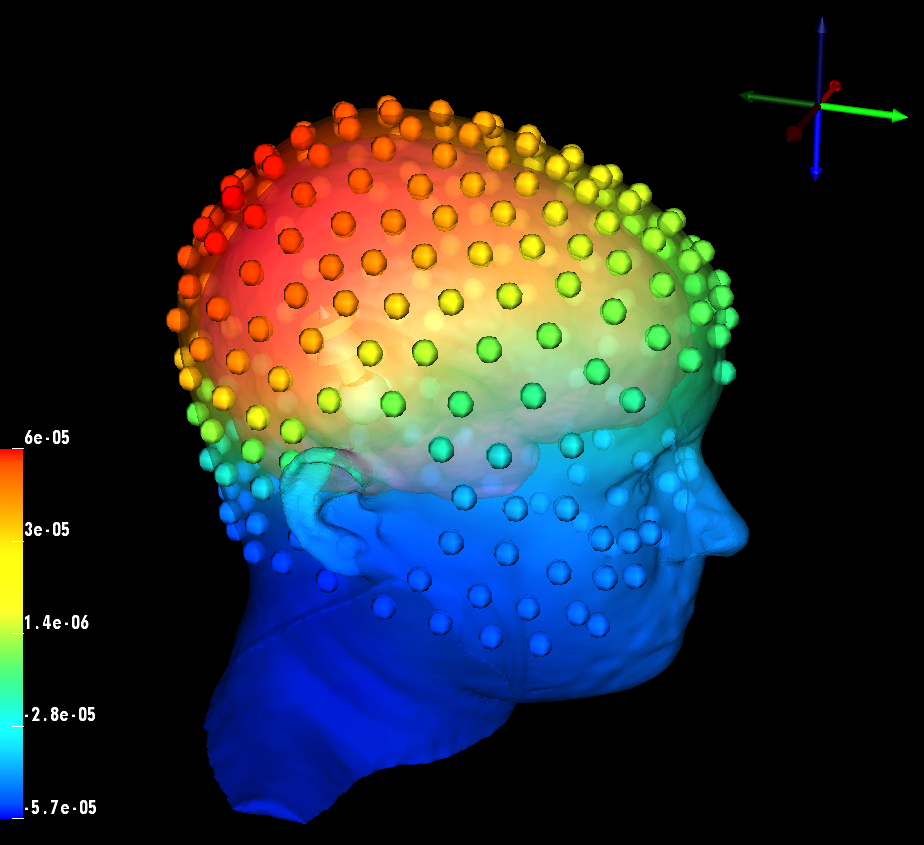
\includegraphics[width=.49\textwidth]{Figures/aniso_dipole}
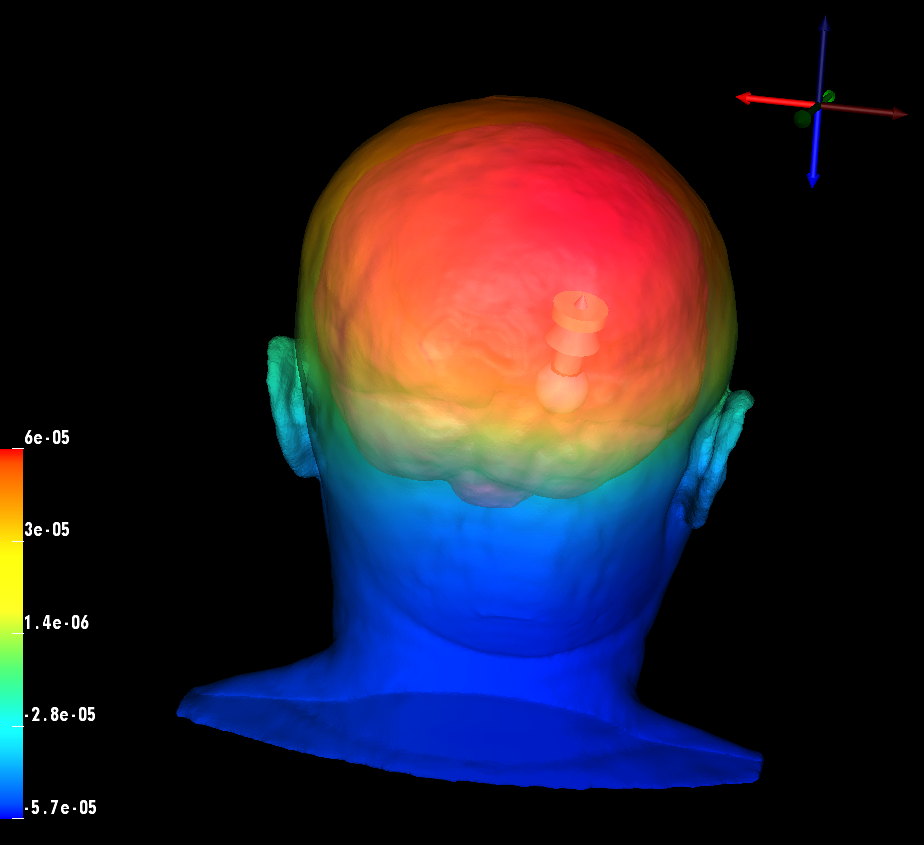
\includegraphics[width=.49\textwidth]{Figures/aniso_dipole_2}
\caption{Anisotropic forward problem solution with dipole source and data mapped onto the head surface and electrodes.}
\label{fig:anisodip}
\end{center}
\end{figure}

\begin{figure}[H]
\begin{center}
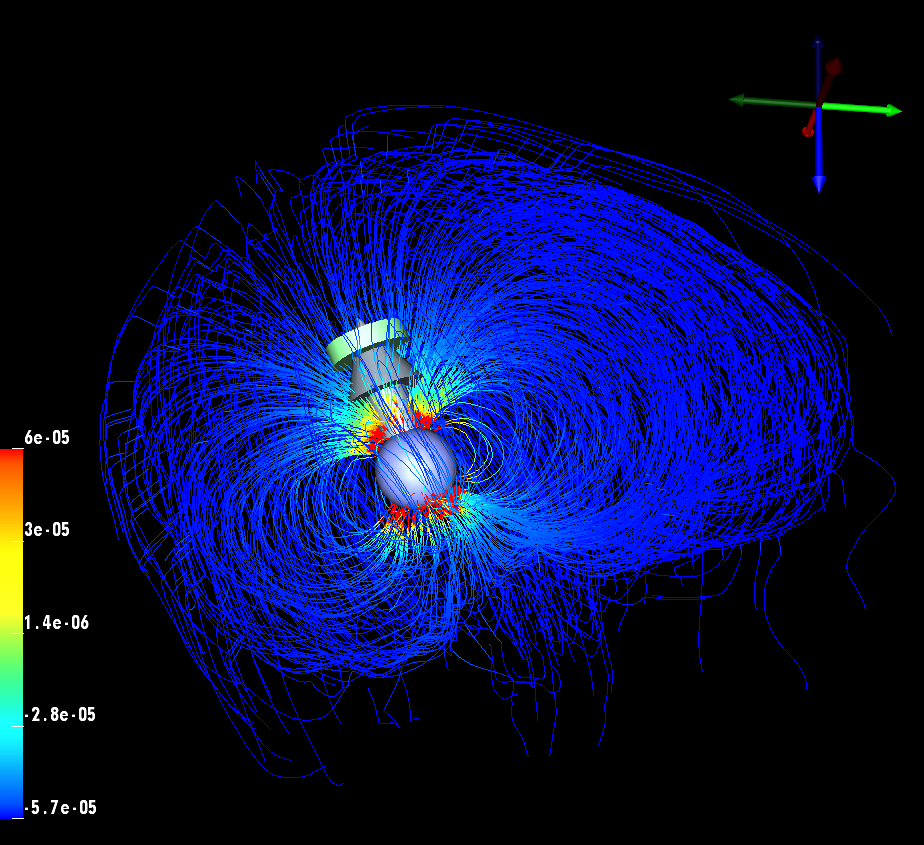
\includegraphics[width=.49\textwidth]{Figures/aniso_streamlines}
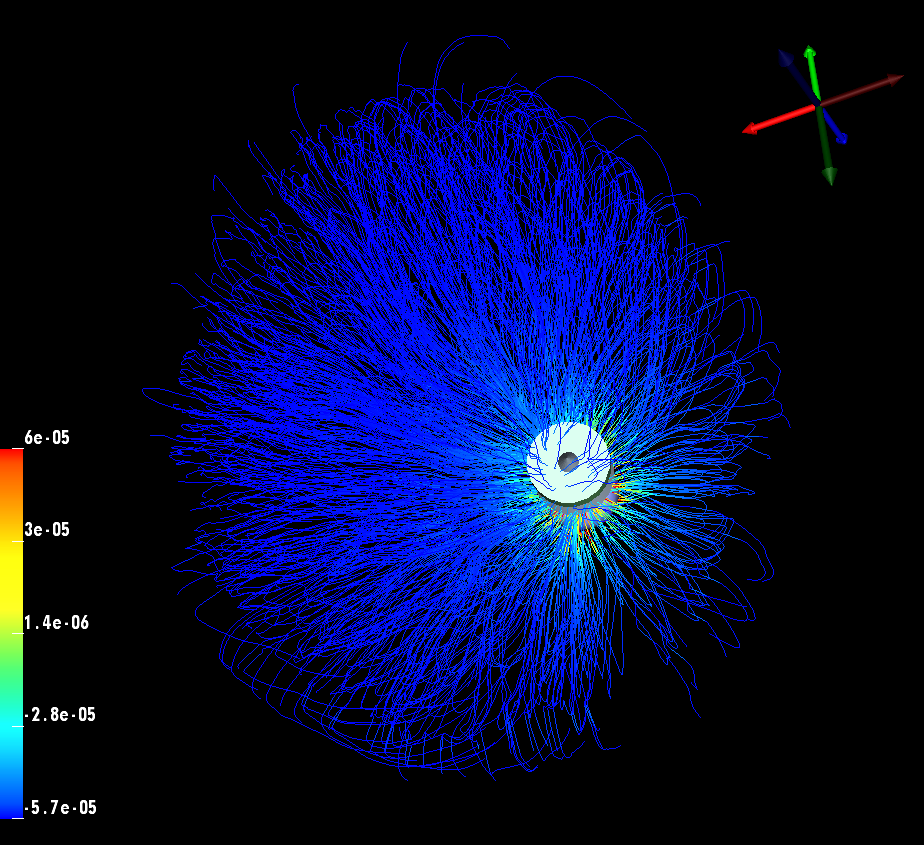
\includegraphics[width=.49\textwidth]{Figures/aniso_streamlines_top}
\caption{Anisotropic streamlines visualization with dipole source.}
\label{fig:anisostream}
\end{center}
\end{figure}

\begin{figure}[H]
\begin{center}
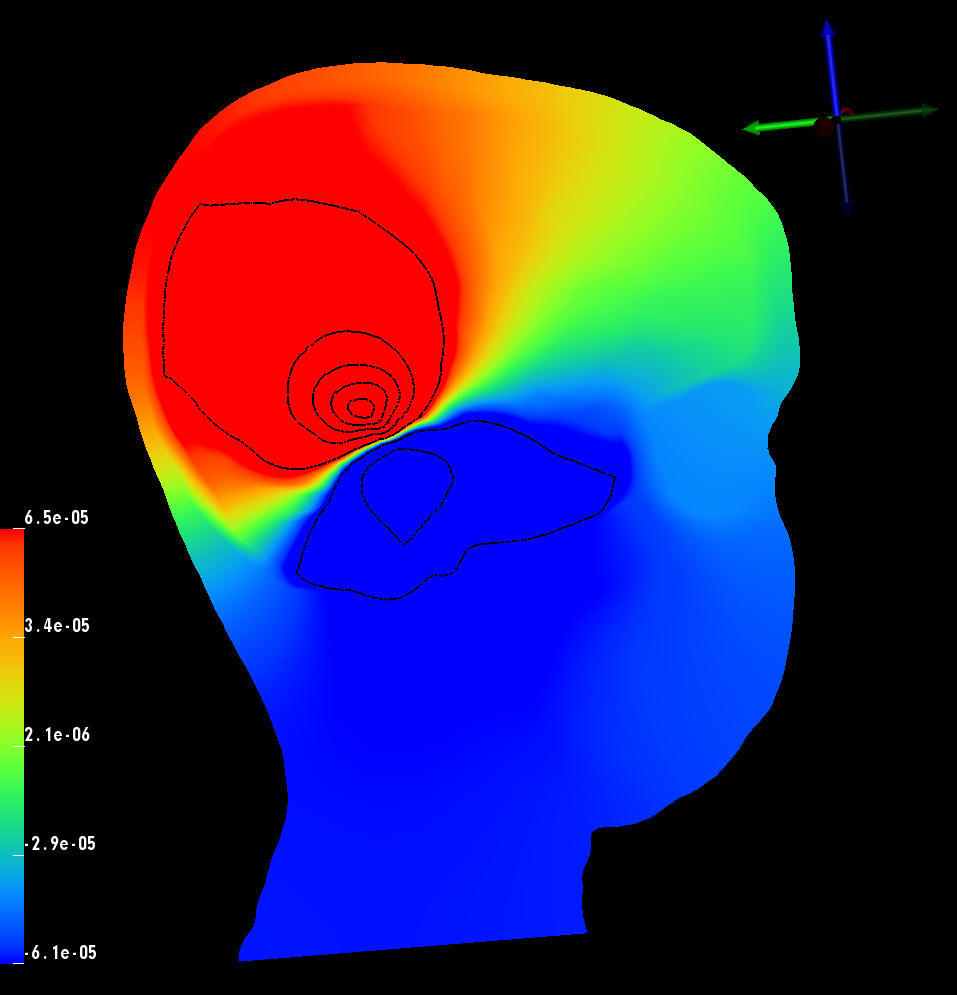
\includegraphics[width=.49\textwidth]{Figures/iso_isolines}
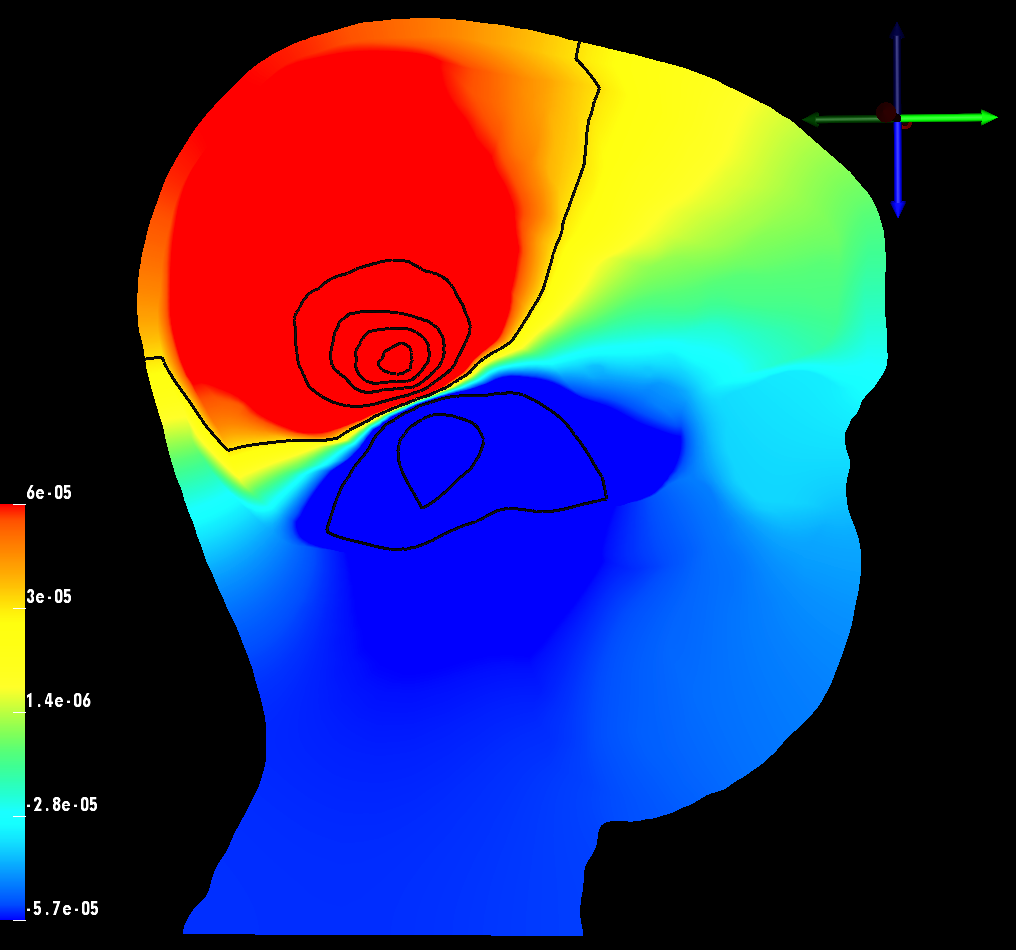
\includegraphics[width = .49\textwidth]{Figures/aniso_isolines}
\caption{Isopotential lines comparison: isotropic white matter conductivity \textit{(left)}, anisotropic white matter conductivity \textit{(right)}.}
\label{fig:isolines}
\end{center}
\end{figure}

\subsection{fMRI Visualization}

fMRI data was a novel imaging datatype for SCIRun. We successfully mapped and visualized the fMRI data onto the cortical surface with a rigid and manual registration to the mesh coordinate space. This mapping network allows for future use of fMRI data in simulations using the SCIRun software package.

\begin{figure}[H]
\begin{center}
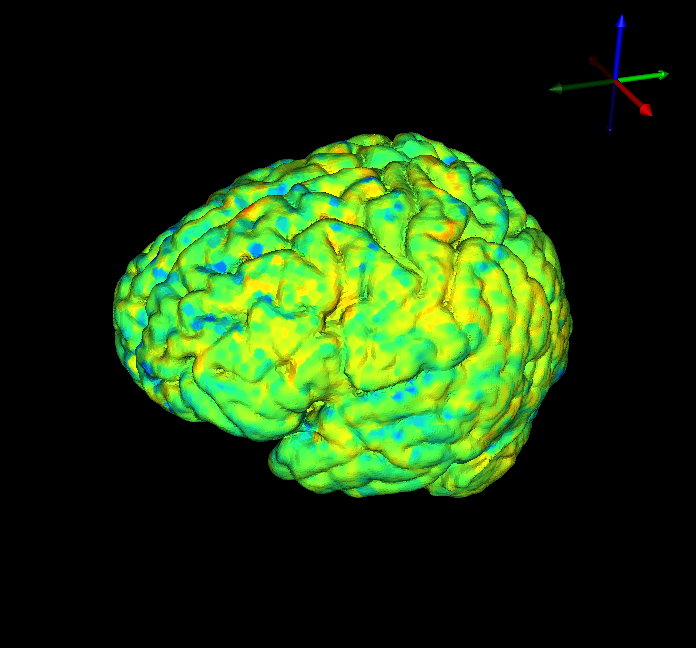
\includegraphics[width=.75\textwidth]{Figures/fmri_1}
\caption{fMRI data mapped onto cortical surface mesh.}
\label{fig:fmrivis}
\end{center}
\end{figure}

\subsection{EEG Visualization}

When using EEG data, the particular application dictates if further processing, filtering, or cutting of the data is necessary. This EEG dataset, taken with 256 electrodes, contained electrodes that require further processing, specifically around the eyes, which was possibly due to the blinking or rolling of the subject's eyes. The bad leads can be corrected or removed with further specific processing or trilinear interpolation.

\begin{figure}[H]
\begin{center}
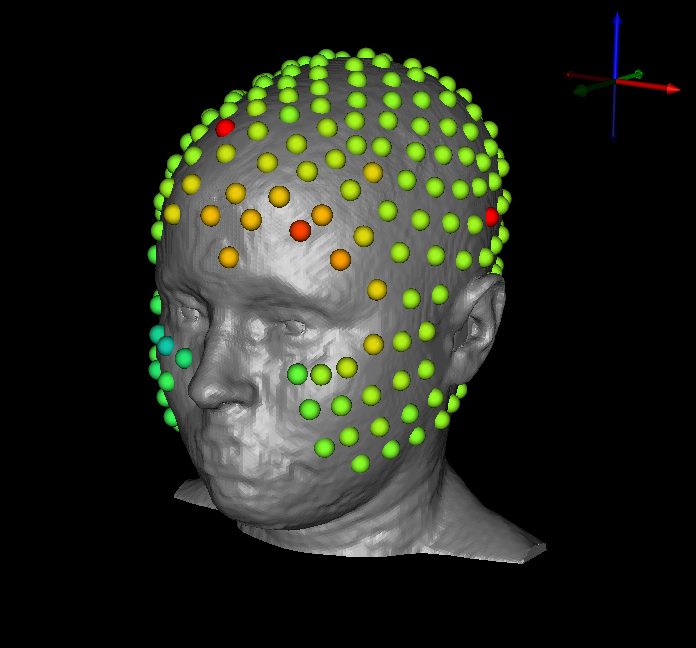
\includegraphics[width=.49\textwidth]{Figures/eeg_1}
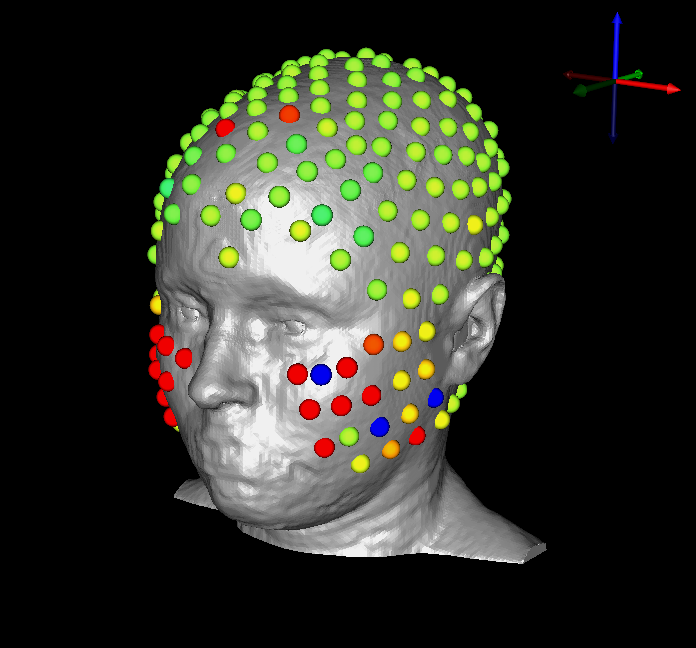
\includegraphics[width=.49\textwidth]{Figures/eeg_2}
\caption{EEG signal visualization with 256 electrodes. Examples of electrodes that require further processing for specific applications - shown in red.}
\label{fig:eegvis}
\end{center}
\end{figure}
The second EEG dataset, taken with 128 electrodes, still has electrodes that require further processing around the eyes. Since the electrodes don't go as far down the cheeks as the other dataset, we do not see as many electrodes that would need further processing. However, the quality of some time steps were too poor for practical use. 

\begin{figure}[H]
\begin{center}
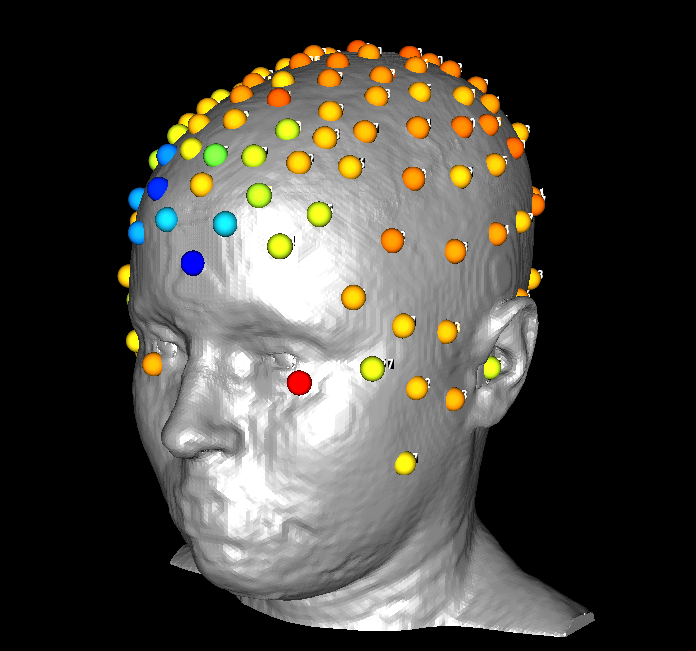
\includegraphics[width=.49\textwidth]{Figures/128_eeg_1}
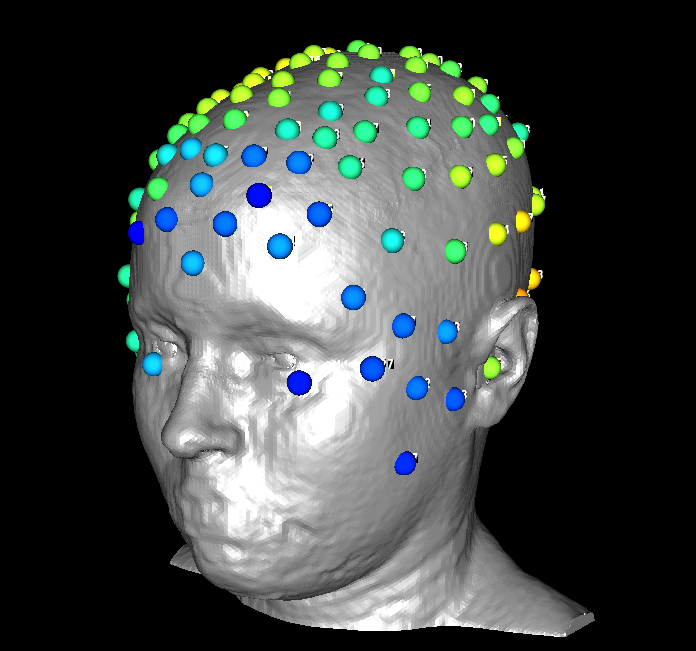
\includegraphics[width=.49\textwidth]{Figures/128_eeg_2}
\caption{EEG signal visualization with 128 electrodes. Examples of electrodes that require further processing for specific applications - shown in red.}
\label{fig:eegvis}
\end{center}
\end{figure}